
\documentclass{gist}

\def\putepsf#1{\centering \parbox{14cm}{\epsfxsize = 14cm \epsfbox{#1}}}
\usepackage{graphicx}

\usepackage{amsmath, amssymb}

% \usepackage{algorithm}
% \usepackage{amsfonts}
% \usepackage{algorithmic}
\AtBeginEnvironment{algorithm}{\setstretch{1.0}}
\usepackage[lofdepth=1]{subfig}
\usepackage[rightcaption]{sidecap}
\usepackage{multirow}
\usepackage{makecell}
% \usepackage{array}

% yoon
\usepackage[ruled,vlined,linesnumbered]{algorithm2e}
\usepackage{etoolbox}
\usepackage{url}

\newcommand\etal{\textit{et~al.\ }}
\newcommand\eg{\textit{e.g.\ }}
\newcommand\ie{\textrm{i.e.\ }}
\newcommand\R{\mathbb{R}}
% yoon

% \usepackage{theorem}
\usepackage{setspace}
\usepackage{appendix}
\usepackage{cite}
\usepackage{csquotes}

\usepackage[colorlinks=true,linkcolor=black,citecolor=black]{hyperref}
% \usepackage[]{hyperref}
% \hypersetup{
%     % bookmarksnumbered=true,
%     %   linkbordercolor=blue,
%     %   filebordercolor=red,
%     %   citebordercolor = green,      
%     %   urlbordercolor=red,
%       %
%       colorlinks=false
%       % linkcolor=blue,
%       % filecolor=blue,
%       % citecolor = blue,      
%       % urlcolor=cyan,
% }

\usepackage{bookmark}
\bookmarksetup{numbered}

\makeatletter
\bookmarksetup{%
  addtohook={%
    \ifnum\toclevel@chapter=\bookmarkget{level}\relax
      \renewcommand*{\numberline}[1]{CHAPTER #1 }%
    \fi
  },
}
\makeatother

\usepackage{cleveref, autonum}

\usepackage{amsthm}
\newtheorem{theorem}{Theorem}[section]
\newtheorem{lemma}{Lemma}[section]
\newtheorem{corollary}{Corollary}[section]
\newtheorem{proposition}{Proposition}[section]
\newtheorem{assumption}{Assumption}[section]
\theoremstyle{remark}
\newtheorem{remark}{Remark}[section]
\theoremstyle{definition}
\newtheorem{definition}{Definition}[section]

%-----------------------------------------------------------------------
% Department code list
% IC - Information and Communications
% IM - Information and Mechatronics
% EC - Electric Engineering and Computer Science
% MS - Materials Science and Engineering
% ME - Mechanical and Robotics Engineering
% AI - Artificial Intelligence Graduate School
% EN - Earth Science and Environmental Engineering
% LS - Life Science
% PH - Physics and Photon Science
% CH - Chemistry
% NA - Nanobio Materials and Electronics
% MD - Biomedical Science and Engineering
% ET - Integrated Technology 에너지 융합 학제
% CT - Integrated Technology 문화기술 융합 학제
% RT - Integrated Technology 지능로봇프로그램

% Department code
%\code{{BS/}{EC}}
%\code{{MS/}{EC}} % 학위와 소속 코드, 초록 페이지에 나타남
\code{{MS/}{AI}}
%-----------------------------------------------------------------------
% Thesis title in English
% Insert \titlebreak where lines are to be separated.  Do not use the LaTeX command '\\'.

%\etitle{Study on Image Segmentation and Action Recognition in Computer Vision}

\etitle{Insert your title}

%\etitle{Study on Segmentation and Recognition for an Image Understanding}
%\etitle{Genetic Programming: \titlebreak New Optimization Tools for Real-World Applications}

%-----------------------------------------------------------------------
% Thesis title in Korean
% Insert \titlebreak where lines are to be separated.  Do not use the LaTeX command '\\'.
%\begin{spacing}{2.0}
\ktitle{한글 제목을 넣으세요}
%\end{spacing}
%-----------------------------------------------------------------------
% Advisor's name in English without a position such as 'Prof.'.
\advisor{Professor Someone}

%-----------------------------------------------------------------------
% Advisor's name in Korean without a position such as 'Prof.'.
\kadvisor{교수님}

%-----------------------------------------------------------------------
% Co-advisor's name in English
% In case there is no co-advisor, comment out the following line with a "%" in the front.
%\coadvisor{My Co-advisor}

%-----------------------------------------------------------------------
% Name of the author in English
\ename{Minseok Seo}

%-----------------------------------------------------------------------
% Name of the author in Korean seperated with '{}'.
\kname{{}{}{}{}{서}{민}{석}} % 한글 이름 7글자까지 가능, 오른쪽 끝에 맞춰서 입력

%-----------------------------------------------------------------------
% Student ID of the author
\studentid{20231115}

%-----------------------------------------------------------------------
% The year of graduation (ex. 1999)
\coveryear{2025}

%-----------------------------------------------------------------------
% The date signed by the advisor.  The first is the month, second the date, and third the year.
\advisorsigndate{June}{20}{2025}

%-----------------------------------------------------------------------
% The date signed by the referees.  The first is the month, second the date, and third the year.
\refereesigndate{June}{20}{2025}

%-----------------------------------------------------------------------
% Names of the referees in English
% For Master's thesis, input the names of the three referees (refereeA thru referee C) in full.
% For Ph.D thesis, input the names of the five referees (refereeA thru referee E) in full.
% For most cases, refereeA is the same as the advisor.

\refereeA{Prof. first prof.}
\refereeB{Prof. second prof.}
\refereeC{Prof. third prof.}
% \refereeD{Prof. fourth prof.}
% \refereeE{Prof. fifth prof.}

%-----------------------------------------------------------------------
% This is the beginning of the thesis.

\dedication{
Dedicated to my family.
}

\begin{document}
%-----------------------------------------------------------------------
% Abstract of the thesis in English.
% Insert the abstract between \begin{eabstract} and \end{eabstract}.
% You can either write the abstract directly here or import a file using the \input command.

%%%%%%%%%%%%%%%%%%%%%%%%%%%%%%%%%%%%%%%%%%
% Abstract by English
%%%%%%%%%%%%%%%%%%%%%%%%%%%%%%%%%%%%%%%%%%

\begin{eabstract}
\begin{spacing}{2.0} % double spacing

%%%%%%%%%%%%%%%%%%%%%%%%%%%%%%%%%%%%%%
% Abstract of the thesis in English
%%%%%%%%%%%%%%%%%%%%%%%%%%%%%%%%%%%%%%

For the practical deployment of autonomous driving systems, high levels of safety and adaptability are essential.
Accordingly, Deep Reinforcement Learning (DRL), which learns and improves driving strategies through trial and error, has gained attention.
However, the reward-driven nature of reinforcement learning may still lead to unsafe or abnormal behavior even after training.
To address this limitation, Constrained Reinforcement Learning (CRL) has been proposed to balance safety and performance.
While CRL typically defines constraints as expected cumulative costs, this formulation does not consider whether constraints are satisfied at each state, making it difficult to ensure state-wise safety.
In this paper, we extend a Lagrangian-based CRL approach by estimating state-wise Lagrangian multipliers, allowing the policy to account for state-level safety.
We evaluate the proposed method in OpenAI's Safety Gym environment and compare its performance with existing Lagrangian-based methods.

\end{spacing}
\end{eabstract}

%-----------------------------------------------------------------------
% Abstract of the thesis in Korean.
% Insert the abstract between \begin{kabstract} and \end{kabstract}.
% You can either write the abstract directly here or import a file using the \input command.

%%%%%%%%%%%%%%%%%%%%%%%%%%%%%%%%%%%%%%%%%%
% Abstract by Korean
%%%%%%%%%%%%%%%%%%%%%%%%%%%%%%%%%%%%%%%%%%

\begin{kabstract}
\begin{spacing}{2.0} % double spacing

%국문초록
%%%%%%%%%%%%%%%%%%%%%%%%%%%%%%%%%%%%%%
% Abstract of the thesis in Korean
%%%%%%%%%%%%%%%%%%%%%%%%%%%%%%%%%%%%%%

한글 초록을 여기에 쓰세요.

\end{spacing}
\end{kabstract}


%-----------------------------------------------------------------------
% Table of contents, list of tables and list of figures.
% Use the \makecontents command to automatically generate the table of content
\makecontents

% In case there is no table, comment out the following line.
% \listtables

% In case there is no figure, comment out the following line.
\listfigures

% In case there is no algorithm, comment out the following line.
% \listalgorithms

%-----------------------------------------------------------------------
% Input the thesis files written in LaTeX.
% The \begin{document} command is not necessary here.
% Refererence and vitae will folllow the main thesis text.
%-----------------------------------------------------------------------
% This is the beginning of the main thesis body.
% Insert Chapter or section or subsection as many as you need.

%%%%%%%%%%%%%%%%%%%%%
% Chapter 1 Introduction
%%%%%%%%%%%%%%%%%%%%%

%%%%%%%%%%%%%%%%%%%%%%%%%%%%%%%%%%%%%%
% DO NOT DELETE FOLLOWING TWO LINES! %
%%%%%%%%%%%%%%%%%%%%%%%%%%%%%%%%%%%%%%
% \begin{spacing}{2.0} % double spacing
\begin{spacing}{1.3} % double spacing
\pagenumbering{arabic}
\setcounter{page}{1}

% you start with the chapter 1

%%%%%%%%%%%%%%%%%%%%%%%%%%%%%%%%
% Chap 1. Introduction
%%%%%%%%%%%%%%%%%%%%%%%%%%%%%%%%

\chapter{Introduction}\label{chapter1}
\section{Introduction} \label{chap1:sec1}

Reinforcement Learning (RL) \cite{RL} is a method for learning an optimal policy through trial and error.
Although its theoretical foundations have been established for several decades, its practical applications were limited by various challenges.
One of the biggest challenges in reinforcement learning is extending it to continuous spaces, which leads to an increase in the dimensionality of state and action spaces.
Due to the exponential growth in the number of possible states and actions, the corresponding rise in computational complexity poses a significant obstacle to learning in high-dimensional environments.
To address this issue, traditional approaches often relied on handcrafted feature engineering to simplify the problem space.
However, designing effective features by hand is both time-consuming and domain-specific, limiting the generalizability of learned policies across different scenarios.
The emergence of deep learning addressed this issue by enabling automatic feature extraction from raw, high-dimensional inputs such as images, sensor data.
This advancement eliminated the need for manual feature design and allowed reinforcement learning agents to operate directly on raw observations.
However, applying deep learning to reinforcement learning introduced another significant challenge: the data collected by agents is highly correlated.
Unlike supervised learning, where training data is typically assumed to be independent and identically distributed (IID), RL agents interact sequentially with the environment, resulting in temporally correlated data.
This violates the IID assumption and can lead to instability and inefficient learning when training neural networks.
A major breakthrough in overcoming these limitations came with the introduction of Deep Q-Network (DQN) \cite{DQN1, DQN2} by DeepMind.
By combining deep neural networks with Q-learning, DQN enabled agents to approximate complex value functions from high-dimensional inputs such as raw pixel images.
This advancement allowed RL agent could achieve human-level performance in a variety of Atari games without relying on handcrafted features.
This success of DQN has led to significant advances in the field of deep reinforcement learning (DRL), such as AlphaGo \cite{AlphaGo} and AlphaZero \cite{AlphaZero} by DeepMind, which demonstrated superhuman performance in board games like Go, Chess, and Shogi.
In addition, OpenAI Five \cite{Five} showcased the power of DRL in complex, multi-agent environments by defeating professional human players in the real-time strategy game Dota 2.
Another notable example is Dactyl \cite{Dactyl}, a robotic hand developed by OpenAI that learned to manipulate physical objects using reinforcement learning trained in simulation and successfully transferred to the real world, highlighting progress in sim-to-real transfer for robotic control.
Despite these impressive achievements, applying reinforcement learning to real-world environments remains challenging.
RL agents typically require a large number of iterations to learn effective policies, often relying on extensive exploration to discover rewarding behaviors.
However, during this exploration process, agents may take unsafe or risky actions that can lead to catastrophic failures—particularly in safety-critical domains such as robotics, autonomous driving, or healthcare.
Moreover, even after training is complete, there is no guarantee that the learned policy will consistently behave safely, especially in unseen or out-of-distribution (OOD) environments.
In particular, transferring policies from simulation to the real world (i.e., the sim-to-real problem) can cause even greater safety concerns when learned behaviors don’t generalize well to the real world.
A key underlying difficulty is the inherent challenge of designing reward functions that reliably induce safe and desirable behaviors across a wide range of situations.

\section{Research Objective}

In this thesis, we investigate how to learn safe policies in reinforcement learning through constrained optimization techniques, focusing on State-wise Constrained Reinforcement Learning (SCRL) \cite{SCRL-survey}, which introduces cost functions to enforce state-wise safety constraints during the learning process.
Among various SCRL approaches, we examine Lagrangian-based methods due to their theoretical simplicity and empirical popularity.
This thesis analyzes the limitations of existing Lagrangian methods in the SCRL setting and empirically examines how specific design choices, including the bias initialization and the learning rate of the Lagrange multiplier network, influence both performance and safety.
We also propose a method, PPO Lagrangian Network, which extends Proximal Policy Optimization to the state-wise constraint setting using a Lagrange multiplier network.
The proposed method is empirically evaluated against existing approaches on a range of tasks from the OpenAI Safety Gym.


\section{Outline of the Thesis}

This thesis is organized as follows:

\begin{itemize}
  \item Chapter \ref{chapter2} provides background on reinforcement learning, including policy gradient methods, constrained reinforcement learning and state-wise constrained reinforcement learning. It also reviews prior work relevant to this thesis.
  \item Chapter \ref{chapter3} introduces the proposed method, PPO Lagrangian Network, which incorporates a state-wise Lagrange multiplier network into the PPO framework. The design and training procedure are detailed, along with comparisons to related methods.
  \item Chapter \ref{chapter4} presents experimental results. We first investigate the influence of key hyperparameters, such as the entropy coefficient $\alpha$, bias initialization, and learning rate of the Lagrange multiplier network. We then evaluate the performance of PPO Lagrangian network across Safety Gym tasks.
  \item Chapter \ref{chapter5} concludes the thesis with a summary of findings and discusses limitations and directions for future research.
\end{itemize}

\end{spacing}

%%%%%%%%%%%%%%%%%%%%%%%%%%%%%%%%%%%%
% Chapter 2 
%%%%%%%%%%%%%%%%%%%%%%%%%%%%%%%%%%%%

% \begin{spacing}{2.0} % double spacing
\begin{spacing}{1.3} % double spacing
%%%%%%%%%%%%%%%%%%%%%%%%%%%%%%%%
% Chap 2. Background
%%%%%%%%%%%%%%%%%%%%%%%%%%%%%%%%

\chapter{Background}\label{chapter2}

%%%%%%%%%%%%%%%%%%%%%%%%%%%%%%%%
\section{Reinforcement Learning} \label{chap2:sec1}
%%%%%%%%%%%%%%%%%%%%%%%%%%%%%%%%

Reinforcement Learning (RL) is a framework in which an agent interacts with an environment and learns a policy to maximize cumulative rewards.
The agent observes the state of the environment, takes actions, and receives rewards based on those actions.
This process is formalized as a Markov Decision Process (MDP) \cite{MDP}, which provides a formal strcuture for modeling decision-making problems.
An MDP is defined by a tuple $\langle \mathcal{S}, \mathcal{A}, P, R, \gamma \rangle$, where $\mathcal{S}$ is the set of states, $\mathcal{A}$ is the set of actions, $P$ is the state transition probability function, $R$ is the reward function, and $\gamma \in [0, 1)$ is the discount factor.
In this thesis, we consider a finite-horizon setting and use the undiscounted return.
The objective of RL is to find an optimal policy $\pi^*$ that maximizes the expected cumulative reward, defined as:
\begin{equation}
  \begin{aligned}
    \theta^* &= \arg\max_\theta J(\theta) \\
    J(\theta) &= \mathbb{E}_{\tau \sim \pi_\theta} \left[\sum^T_{t = 0} r_t \right]
  \end{aligned}
\end{equation}
The policy $\pi_\theta$ is assumed to be a differentiable function parmeterized by $\theta$, denoted as $\pi_\theta(a|s)$, which represents the probability of taking ation $a$ given state $s$.
The expectation $\mathbb{E}_{\tau \sim \pi_\theta}$ is taken over the trajectories $\tau = (s_0, a_0, r_0, s_1, a_1, r_1, \ldots, s_T)$ generated by following the policy $\pi_\theta$.


\subsection{Policy Gradient Methods} \label{chap2:sec2}

Since the policy is differentiable, its gradient can be expressed using the likelihood ratio trick:
\begin{equation}
  \begin{aligned}
    \nabla_\theta \pi_\theta(s, a)
    &= \pi_\theta(s, a) \frac{\nabla_\theta \pi_\theta(s, a)}{\pi_\theta(s, a)} \\
    &= \pi_\theta(s, a) \nabla_\theta \log \pi_\theta(s, a)
  \end{aligned}
\end{equation}
This term $\nabla_\theta \log \pi_\theta(s, a)$ is referred to as the score function.
Although we previously defined the objective function $J(\pi_\theta)$ as the expected cumulative reward, we now consider a simplified case to facilitate explanation.
A one-step MDP, in which the agent takes an action from the initial state, receives a reward, and the episode terminates immediately.
Then, the objective function can be written as ($d$ is the initial state distribution):
\begin{equation}
  \begin{aligned}
    J(\theta)
    &= \mathbb{E}_{\pi_\theta}[r] \\
    &= \sum_{s \in \mathcal{S}} d(s) \sum_{a \in \mathcal{A}} \pi_\theta(s, a) R_{s ,a}
  \end{aligned}
\end{equation}
The gradient of the objective function can be computed as follows:
\begin{equation}
  \begin{aligned}
    \nabla_\theta J(\theta)
    &= \sum_{s \in \mathcal{S}} d(s) \sum_{a \in \mathcal{A}} \nabla_\theta \pi_\theta(s, a) R_{s, a} \\
    &= \sum_{s \in \mathcal{S}} d(s) \sum_{a \in \mathcal{A}} \pi_\theta(s, a) \nabla_\theta \log \pi_\theta(s, a) R_{s, a} \\
    &= \mathbb{E}_{\pi_\theta} [\nabla_\theta \log \pi_\theta(s, a) r]
  \end{aligned}
\end{equation}
The policy gradient theorem generalizes this result to multi-step MDP, where the objective function is defined as the expected cumulative reward over multiple time steps.
In other words, it replaces the instantaneous reward $r$ with the long-term value $Q^{\pi_\theta} (s, a)$, the action value function.
\begin{theorem}[Policy Gradient Theorem] \label{chap2:thm:pg}
  \begin{equation}
    \nabla_\theta J(\theta) = \mathbb{E}_{\pi_\theta} [\nabla_\theta \log \pi_\theta(s, a) Q^{\pi_\theta}(s, a)]
  \end{equation}
\end{theorem}

\subsubsection{REINFORCE}

In practice, the exact action value function $Q^{\pi_\theta} (s, a)$ is typically unknown.
Accordingly, the estimated return $G_t$ can be used as an approximation of the action value function.
In other words, the action value function $Q^{\pi_\theta} (s, a)$ can be replaced with the return $G_t$ from real sample trajectories using the Monte Carlo method.
\begin{equation}
  \nabla_\theta J(\theta) = \mathbb{E}_{\pi_\theta}[\nabla_\theta \log \pi_\theta(s, a) G_t]
\end{equation}
This leads to the Monte-Carlo policy gradient method, commonly known as REINFORCE \cite{REINFORCE}.
However, REINFORCE suffers from high variance in the gradient estimates, due to its reliance on a full trajectory.

\subsubsection{Actor-Critic}

A common approach to reducing the variance is to use a critic approximates the action value function, $Q_\phi(s, a) \approx Q^{\pi_\theta}(s, a)$.
\begin{equation}
  \nabla_\theta J(\theta) = \mathbb{E}_{\pi_\theta} [\nabla_\theta \log \pi_\theta(s, a) Q_\phi(s, a)]
\end{equation}
This is the basic idea of the Actor-Critic methods.
Actor updates the policy parameters $\theta$ and a critic updates the value function parameters $\phi$.

\subsubsection{Advantage Actor-Critic}
To further reduce the variance, we can introduce a baseline function $B(s)$.
Importantly, subtracting a baseline from the action value function does not change the gradient because its gradient is zero.
\begin{equation}
  \begin{aligned}
    \mathbb{E}_{\pi_\theta} [\nabla_\theta \log \pi_\theta(s, a) B(s)]
    &= \sum_{s \in \mathcal{S}} d(s) \sum_{a \in \mathcal{A}} \pi_\theta(s, a) \nabla_\theta \log \pi_\theta(s, a) B(s) \\
    &= \sum_{s \in \mathcal{S}} d(s) \sum_{a \in \mathcal{A}} \nabla_\theta \pi_\theta(s, a) B(s) \\
    &= \sum_{s \in \mathcal{S}} d(s) B(s) \nabla_\theta \sum_{a \in \mathcal{A}} \pi_\theta(s, a) \\
    &= 0
  \end{aligned}
\end{equation}
Therefore, subtracting a baseline function from the action value function not only leaves the gradient unchanged but also reduces its variance.
\begin{equation} \label{chap2:eq:pg_adv}
  \begin{aligned}
    A^{\pi_\theta}(s, a) &= Q^{\pi_\theta}(s, a) - V^{\pi_\theta}(s) \\
    \nabla_\theta J(\theta) &= \mathbb{E}_{\pi_\theta} [\nabla_\theta \log \pi_\theta(s, a) A^{\pi_\theta}(s, a)]
  \end{aligned}
\end{equation}
However, since the exact advantage function is generally inaccessible, both the action value function $Q^{\pi_\theta}(s, a)$ and the value function $V^{\pi_\theta}(s)$ must be approximated.
One common approach is to use the temporal difference (TD) error $\delta^{\pi_\theta}$, which is an unbiased estimator of the advantage function.
To summarize, the policy gradient has many equivalent formulations:
\begin{equation}
  \begin{aligned}
    \nabla_\theta J(\theta)
    &= \mathbb{E}_{\pi_\theta}[\nabla_\theta \log \pi_\theta(s, a) v_t] &\quad \text{REINFORCE} \\
    &= \mathbb{E}_{\pi_\theta}[\nabla_\theta \log \pi_\theta(s, a) Q_\phi(s, a)] &\quad \text{Q Actor-Critic} \\
    &= \mathbb{E}_{\pi_\theta}[\nabla_\theta \log \pi_\theta(s, a) A^{\pi_\theta}(s, a)] &\quad \text{Advantage Actor-Critic} \\
    &= \mathbb{E}_{\pi_\theta}[\nabla_\theta \log \pi_\theta(s, a) \delta^{\pi_\theta}] &\quad \text{TD Actor-Critic}
  \end{aligned}
\end{equation}

\subsubsection{Proximal Policy Optimization (PPO)}

The methods introduced above are all on-policy: training samples are collected using the same policy that we want to optimize.
However, on-policy methods can be inefficient in terms of sample usage and may suffer from instability due to large updates.
Proximal Policy Optimization (PPO) \cite{PPO} addresses these issue by incorporating importance sampling to reuse data collected from the old policy and introducing a clipped surrogate objective function to prevent large policy updates that may cause divergence.
Based on the Advantage Actor-Critic formulation Eq. \ref{chap2:eq:pg_adv}, the policy gradient can be interpreted as optimizing the following objective function:
\begin{equation}
  J(\theta) = \mathbb{E}_{\pi_\theta}[\log \pi_\theta(s, a) A^{\pi_\theta}(s, a)]
\end{equation}
This formulation assumes that data is collected from the current policy.  
However, in order to improve sample efficiency by reusing data from a previous policy $\pi_{\theta_\text{old}}$, we can apply importance sampling.
So, the objective function can be rewritten as:
\begin{equation}
  J^{\text{TRPO}}(\theta) = \mathbb{E}_{\pi_{\theta_\text{old}}} \left[ \frac{\pi_\theta (s, a)}{\pi_{\theta_\text{old}}(s, a)}A^{\pi_{\theta_\text{old}}}(s, a) \right]
\end{equation}
This objective was introduced in Trust Region Policy Optimization (TRPO) \cite{TRPO}, the predecessor of PPO.
In this formulation, $r(\theta) = \frac{\pi_\theta (s, a)}{\pi_{\theta_\text{old}}(s, a)}$ represents the probability ratio between old and new policies.
While, this allows us to reuse data from the old policy, maximizing this objective without any constraint can lead to large updates and unstable training.
To prevent such instability, PPO imposes the constraint by forcing $r(\theta)$ to stay within a small interval $[1 - \epsilon, 1 + \epsilon]$.
\begin{equation}
  J^{\text{PPO}}(\theta) = \mathbb{E}_{\pi_{\theta_\text{old}}} \left[ \min \left( r(\theta) A^{\pi_{\theta_\text{old}}}(s, a), \text{clip}(r(\theta), 1 - \epsilon, 1 + \epsilon) A^{\pi_{\theta_\text{old}}}(s, a) \right) \right]
\end{equation}
The function $\text{clip}(r(\theta), 1 - \epsilon, 1 + \epsilon)$ clips the probability ratio to the range $[1 - \epsilon, 1 + \epsilon]$.
Therefore, the objective function takes the minimum one between the original value and the clipped value.
This ensures that the policy update does not deviate too far from the old policy, thus stabilizing the training process.

%%%%%%%%%%%%%%%%%%%%%%%%%%%%%%%%
\subsection{Off-Policy Gradient Methods} \label{chap2:sec3}
%%%%%%%%%%%%%%%%%%%%%%%%%%%%%%%%

Off-policy methods allow the agent to learn from data collected by a different policy called the behavior policy.
As a result, the off-policy approach improves sample efficiency by enabling the reuse of past experiences and enhances exploration by allowing the agent to learn from data collected by a behavior policy.
In order to apply off-policy learning within the policy gradient framework, we can incorporate importance sampling into the policy gradient Theorem \ref{chap2:thm:pg}.
\begin{equation}
  \begin{aligned}
    \nabla_\theta J(\theta)
    &= \mathbb{E}_{\tau \sim \pi_\theta} [\nabla_\theta \log \pi_\theta(s, a) Q^{\pi_\theta}(s, a)] \\
    &= \mathbb{E}_{\tau \sim \beta} \left[ \frac{\pi_\theta(s, a)}{\beta(s, a)} \nabla_\theta \log \pi_\theta(s, a) Q^{\pi_\theta}(s, a) \right]
  \end{aligned}
\end{equation}
This allows to estimate the gradient using samples generated by a behavior policy $\beta$ instead of the current policy $\pi_\theta$.

\subsubsection{Soft Actor-Critic (SAC)} \label{chap2:sec3:sac}

Soft Actor-Critic (SAC) \cite{SAC1, SAC2, SAC3} is an off-policy actor-critic model.
In SAC, the policy is trained with the objective of maximizing the expected return and the entropy of the policy.
\begin{equation}
  J(\theta) = \mathbb{E}_{\tau \sim \pi_\theta} \left[ \sum^T_{t = 0} (r_t + \alpha \mathcal{H}(\pi_\theta(\cdot|s_t))) \right]
\end{equation}
\begin{equation}
  \mathcal{H}(\pi_\theta(\cdot|s_t)) = \mathbb{E}_{a_t \sim \pi_\theta}[-\log \pi_\theta(a_t|s_t)]
\end{equation}
where $\mathcal{H}(\cdot)$ is the entropy measure and $\alpha$ controls how important the entropy term is relative to the reward.
Entropy maximization leads to policies that can explore more and capture multiple modes of near-optimal strategies.
If there exist multiple options that seem equally good, the policy should assign each of them an equal probability.
In the SAC algorithm, the policy is updated through the soft policy iteration.
First, the policy evaluation step of soft policy iteration computes the soft Q-value:
\begin{equation}
  Q^{\pi_\theta}(s, a) = \mathbb{E}_{\tau \sim \pi_\theta} \left[ \sum^T_{t = 0} \left(r_t + \alpha \mathcal{H}(\pi_\theta(\cdot|s_t))\right) \Big| s_0 = s, a_0 = a \right]
\end{equation}
Then, the policy improvement step updates the policy to minimize the KL-divergence:
\begin{equation}
  \begin{aligned}
    J(\theta)
    &= \mathbb{E}_{s_t \sim \mathcal{D}} \left[ D_\text{KL} \left( \pi_\theta(\cdot|s_t) \Big|\Big| \frac{\exp(Q_\theta(s_t, \cdot))}{z_\theta(s_t)} \right) \right] \\
    &= \mathbb{E}_{s_t \sim \mathcal{D}} \left[ \mathbb{E}_{a_t \sim \pi_\theta} [\alpha \log (\pi_\theta(a_t|s_t)) - Q_\phi(s_t, a_t)] \right]
  \end{aligned}
\end{equation}

%%%%%%%%%%%%%%%%%%%%%%%%%%%%%%%%
\section{Constrained Reinforcement Learning} \label{chap2:sec4}
%%%%%%%%%%%%%%%%%%%%%%%%%%%%%%%%

Constrained Reinforcement Learning (CRL) extends the standard RL framework by incorporating constraints into the learning process.
CRL is formalized as a Constrained Markov Decision Process (CMDP) \cite{CMDP}, which is defined by a tuple $\langle \mathcal{S}, \mathcal{A}, \mathcal{P}, \mathcal{R}, \mathcal{C}, \gamma \rangle$.
Here, $\mathcal{C}$ is the cost functions associated with the constraints.
The feasible policy set in a CMDP is given by:
\begin{equation}
  \Pi_C = \{\pi: J_{c_i}(\pi) \leq d_i, \quad i = 1, \cdots, k\}
\end{equation}
where $J_{c_i}(\pi)$ is a cost-based constraint function defined the expected cumulative cost, and $d_i$ is the threshold for the $i$-th constraint.
The objective of CRL is to find an optimal policy that maximizes the expected cumulative reward while satisfying the constraints.
In the context of policy gradient methods, the constrained optimization problem can be formulated as follows:
\begin{equation} \label{chap2:eq:crl-objective}
  \begin{aligned}
    \theta^* &= \arg\max_\theta J(\theta) \\
    J(\theta) &= \mathbb{E}_{\tau \sim \pi_\theta} \left[ \sum^T_{t = 0} r_t \right] \; \text{subject to} \; \mathbb{E}_{\tau \sim \pi_\theta} \left[ \sum^T_{t = 0} c_t \right] \leq d
  \end{aligned}
\end{equation}

\subsection{Lagrangian Method}

Constrained optimization problem defined in Eq. \ref{chap2:eq:crl-objective} can be solved using various methods.
In this thesis, however, we consider only the Lagrangian method.
By applying Lagrangian relaxation, the constrained optimization problem can be transformed into an unconstrained optimization problem, in which the constraint is incorporated into the objective function using a Lagrange multiplier $\lambda$.
\begin{equation}
  \begin{aligned}
    \theta^* &= \arg\max_\theta \mathcal{L}(\theta, \lambda) \\
    \mathcal{L}(\theta, \lambda) &= \mathbb{E}_{\tau \sim \pi_\theta} \left[ \sum^T_{t = 0} r_t \right] - \lambda \left( \mathbb{E}_{\tau \sim \pi_\theta} \left[ \sum^T_{t = 0} c_t \right] - d \right)
  \end{aligned}
\end{equation}
The Lagrange multiplier $\lambda$ is a non-negative scalar that adjusts the trade-off between maximizing the expected cumulative reward and satisfying the constraints.

\subsection{Related Work: PPO Lagrangian}

PPO Lagrangian is an adaptation of PPO to the CRL setting by incorporating the Lagrangian method \cite{PPO-Lagrangian}.
Thus, the objective function of PPO Lagrangian can be written as:
\begin{equation} \label{chap2:eq:ppo_lag}
  \begin{aligned}
    J^{\text{PPO-Lag}}(\theta) = \mathbb{E}_{\pi_{\theta_\text{old}}} \Big[ &\min \big( r(\theta) A^{\pi_{\theta_\text{old}}}(s, a), \text{clip}(r(\theta), 1 - \epsilon, 1 + \epsilon) A^{\pi_{\theta_\text{old}}}(s, a) \big) \\
    &- \lambda r(\theta) A^{\pi_{\theta_\text{old}}}_c \Big]
  \end{aligned}
\end{equation}
where $\lambda$ is the Lagrange multiplier that adjusts the trade-off between the reward and the cost.
$A^{\pi_{\theta_\text{old}}}_c$ is the advantage function for the cost.
The Lagrange multiplier $\lambda$ is updated iteratively during training to ensure the constraint is satisfied.
The update of the Lagrange multiplier depends on whether the empirical cumulative cost exceeds the threshold $d$.
Specifically, the empirical cumulative cost is computed as:
\begin{equation}
  \hat{J}_c = \frac{1}{N} \sum^N_{i = 1} \sum^T_{t = 0}  c^{(i)}_t
\end{equation}
where $N$ is the number of sampled episodes, and $c^{(i)}_t$ denotes the cost received at time step $t$ in the $i$-th episode.
The Lagrange multiplier $\lambda$ is updated via gradient ascent:
\begin{equation}
  \lambda \leftarrow \left[ \lambda + \beta\left( \hat{J}_c - d \right) \right]_+
\end{equation}
where $\beta$ is the leraning rate, and $[\cdot]_+$ denotes clipped to be non-negative.
This update increases $\lambda$ when the empirical cost exceeds the threshold $d$, encouraging the policy to reduce the cost in subsequent updates.
The overall structure of PPO Lagrangian is illustrated in Fig.~\ref{chap2:fig:ppo_lag}.
The agent interacts with the environment by taking actions generated from the actor network, thereby collecting trajectories. 
Using the actual rewards and costs obtained from the trajectories, the value functions are updated, and both reward and cost advantages are computed. 
The Lagrange multiplier is updated based on the cost returns from the trajectories. 
Finally, the policy is updated using the reward advantage, cost advantage, and the Lagrange multiplier according to Equation~\ref{chap2:eq:ppo_lag}.

\begin{figure*}[t]
  \centering
  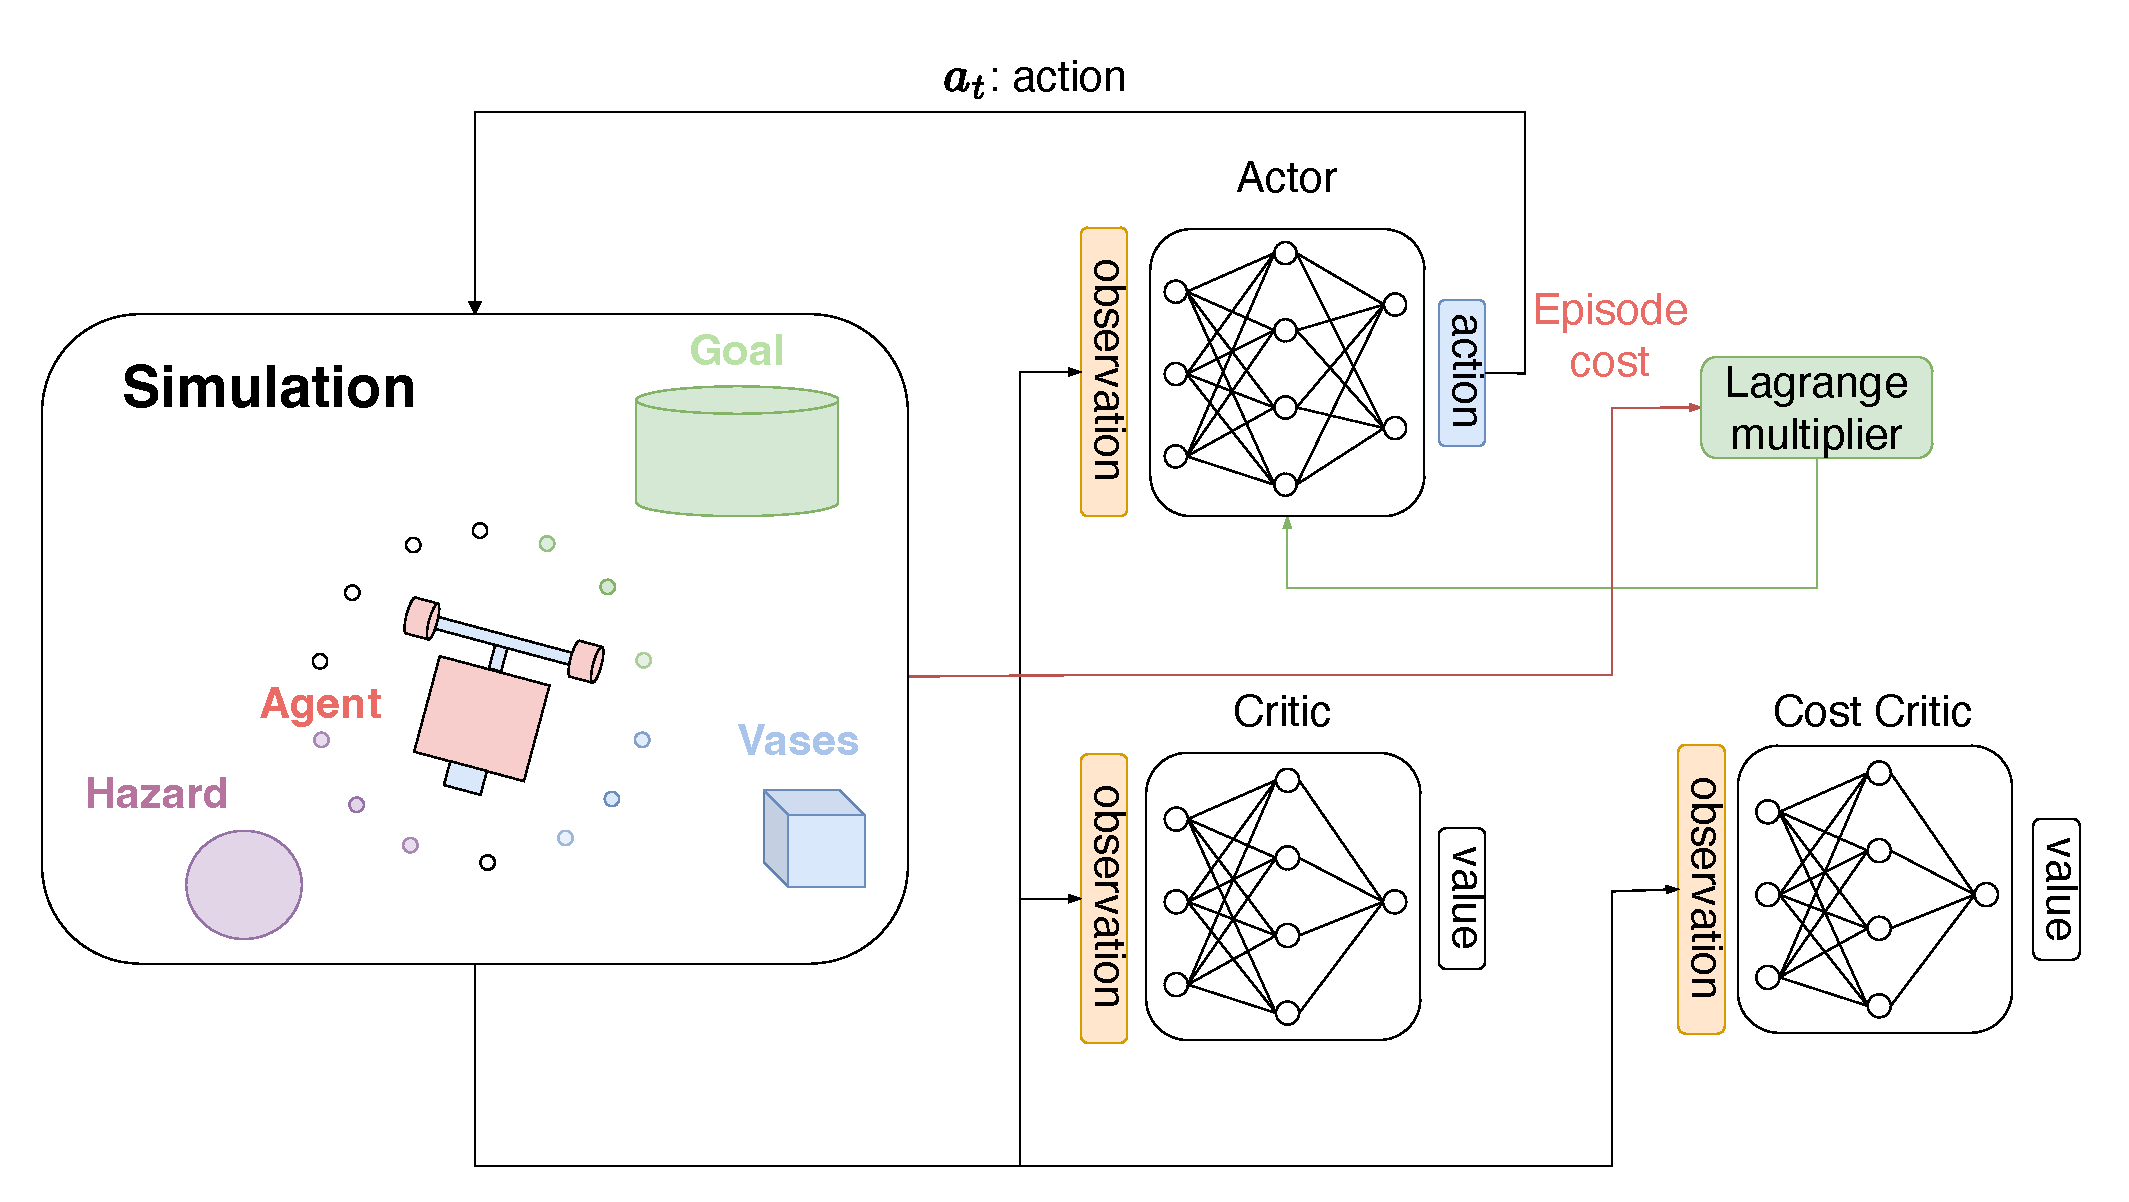
\includegraphics[width=1.0\textwidth]{imgs/chap2/ppo_lag.pdf}
  \caption{Structure of PPO Lagrangian}
  \label{chap2:fig:ppo_lag}
\end{figure*}

%%%%%%%%%%%%%%%%%%%%%%%%%%%%%%%%
\section{State-wise Constrained Reinforcement Learning} \label{chap2:sec5}
%%%%%%%%%%%%%%%%%%%%%%%%%%%%%%%%

State-wise Constrained Reinforcement Learning (SCRL) is a variant of CRL that imposes constraints at the state level.
CRL considers the cumulative cost over the entire trajectory, while SCRL focuses on the cost at each transition.
SCRL is formalized as a State-wise Constrained Markov Decision Process (SCMPD), it is quite similar to CMDP, but SCMDP enforces the constraint for every state action trasition satisfies a hard constraints.
The objective of SCRL is to find an optimal policy that maximizes the expected cumulative reward while satisfying the state-wise constraints.
\begin{equation}
  \begin{aligned}
    \pi^* &= \arg\max_{\pi_\theta} J(\theta) \\
    J(\theta) &= \mathbb{E}_{\tau \sim \pi_\theta} \left[ \sum^T_{t = 0} r_t \right] \; \text{subject to} \; \mathbb{E}_{\tau \sim \pi_\theta}  [c(s, a)] \leq w, \quad \forall s \in S
  \end{aligned}
\end{equation}

\subsection{Related Work: Feasible Actor-Critic} \label{chap2:sec5:fac}

Feasible Actor-Critic (FAC) is an extension of the Soft Actor-Critic algorithm to the SCRL setting \cite{FAC}.
In FAC, the state-wise constraint is enforced via a cost action-value function, formulated as:
\begin{equation}
  Q^{\pi_\theta}_c(s, a) = \mathbb{E}_{\tau \sim \pi_\theta}\left[\sum^T_{t = 0} c_t |s_0 = s, a_0 = ~a \right] \leq w
\end{equation}
The objective function of FAC is defined as:
\begin{equation} \label{chap2:eq:fac}
  \begin{aligned}
    J^{\text{FAC}}(\theta) = \mathbb{E}_{s_t \sim \mathcal{D}} \Big[ \mathbb{E}_{a_t \sim \pi_\theta} \big[ 
    &\alpha \log(\pi_\theta(a_t|s_t)) - Q_\phi(s_t, a_t) \\
    &+ \lambda_\xi(s_t)\left( Q_{\phi_c}(s_t, a_t) - w \right) 
    \big] \Big]
  \end{aligned}
\end{equation}
where $Q_{\phi_c}$ is the cost action-value function, and $\lambda_\xi$ is the Lagrange multiplier network, which estimate the Lagrange multiplier for each state.
The update of the Lagrange multiplier network depends on whether the cost action-value function exceeds the threshold $w$.
\begin{equation}
  J_\lambda(\xi) = \mathbb{E}_{s_t \sim \mathcal{D}} \left[ \mathbb{E}_{a_t \sim \pi_\theta} \left[ \lambda_\xi(s_t) \left( Q_{\phi_c}(s_t, a_t) - w \right) \right] \right]
\end{equation}
Fig.~\ref{chap2:fig:fac} illustrates the architecture of Feasible Actor-Critic (FAC). 
Since FAC is an off-policy algorithm, samples collected during the rollout phase are stored in a replay buffer, and mini-batches are drawn from it to update the actor, critics, and Lagrange multiplier network. 
The environment-provided reward and cost are used to update their respective Q-functions.
Using the reward and cost values estimated by the critic networks, together with the Lagrange multiplier computed from the Lagrange multiplier network, the policy is updated according to Equation~\ref{chap2:eq:fac}. 
The Lagrange multiplier network is updated based on the cost values estimated by the cost Q-function.
\begin{figure*}[h]
  \centering
  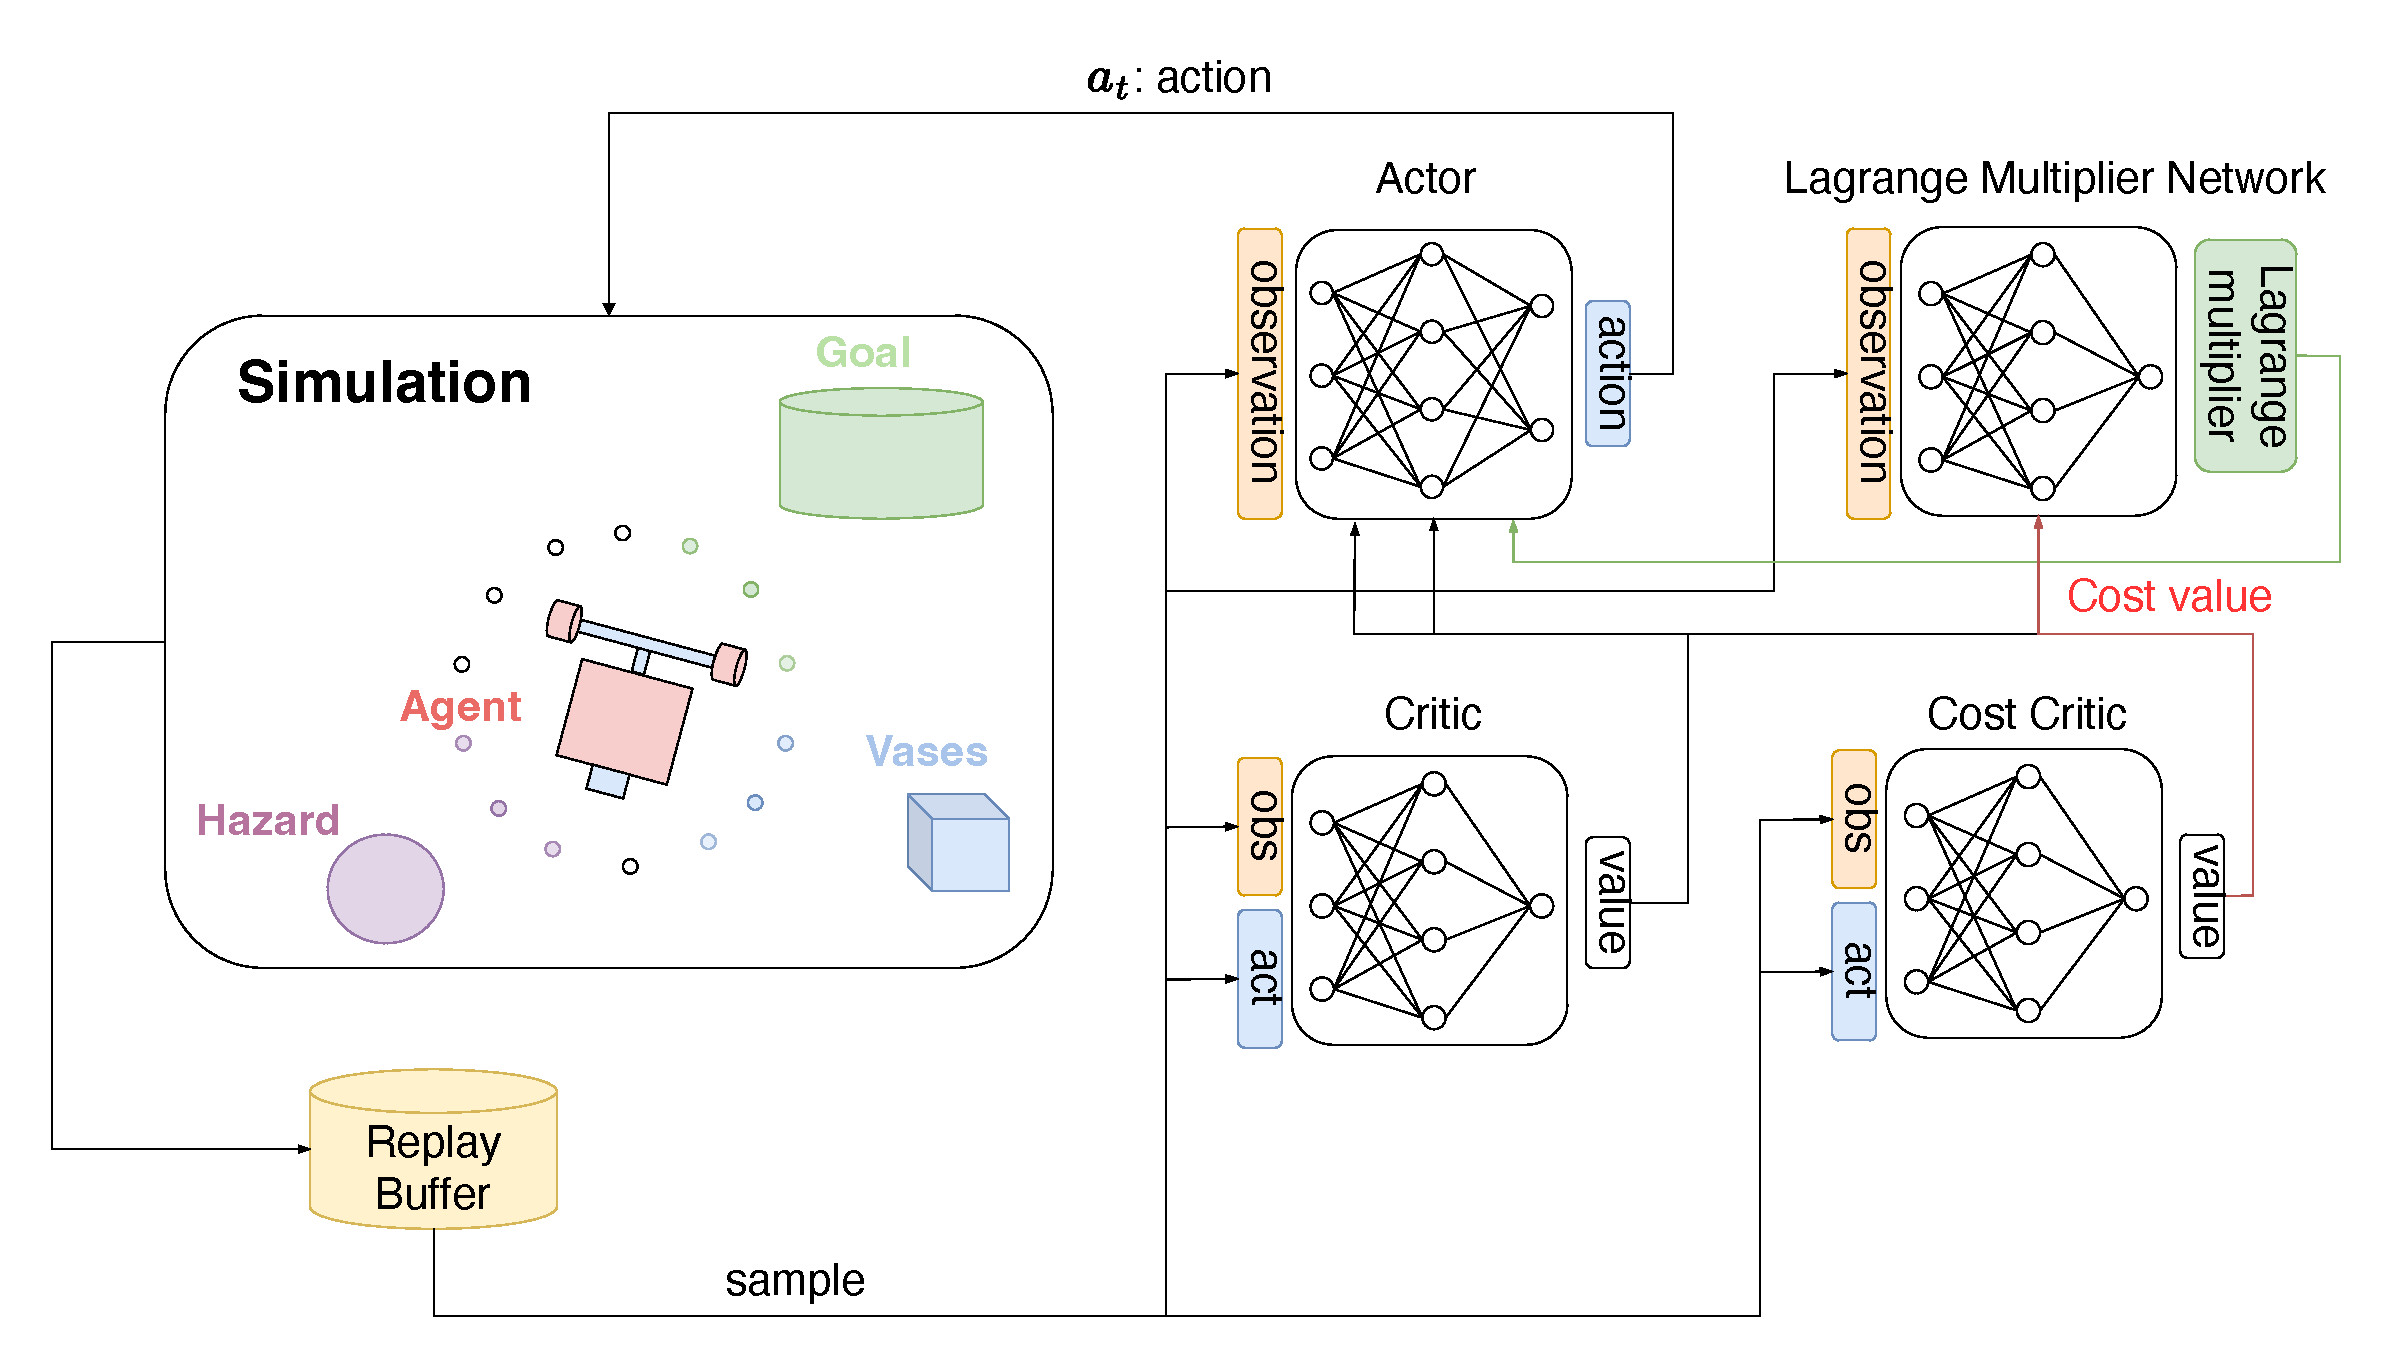
\includegraphics[width=1.0\textwidth]{imgs/chap2/fac.pdf}
  \caption{Structure of Feasible Actor-Critic}
  \label{chap2:fig:fac}
\end{figure*}

\noindent Although FAC contributes by proposing a framework that leverages a Lagrange multiplier network to address state-wise safety in policy learning, it has several limitations.
\begin{itemize}
  \item 
  Soft Actor-Critic (SAC) encourges exploration and promotes diverse action selection by adjusting the temperature parameter $\alpha$. 
  However, this objective can conflict with the constraint penalty term, which pushes the policy toward satisfying constraints. 
  As a result, it becomes more difficult for the policy consistently satisfy the constraints.
  \item 
  Instead of using the empirical cost values, FAC relies on a cost value estimated by the cost action-value function $Q_{\phi_c}(s, a)$.
  This introduces instability in the update of the Lagrange multiplier network due to potentially inaccurate cost estimates, which in turn can lead to unreliable policy updates.
\end{itemize}

\end{spacing}

      
%%%%%%%%
% Add more chapters if you wants
%%%%%%%%


%---------
% summary
%---------
\begin{spacing}{2.0}

\summary

This thesis studies how to train policies to satisfy state-wise safety using state-wise constrained reinforcement learning.
We focus on Lagrangian-based approaches and identify their key limitations, particularly with respect to stability and convergence.
To address these challenges, we propose PPO Lagrangian Network, an extension of Proximal Policy Optimization that incorporates a Lagrange multiplier network to dynamically enforce safety constraints at the state level.
Extensive experiments on the OpenAI Safety Gym benchmark show that proposed method achieves more stable and reliable constraint satisfaction than existing approaches such as PPO Lagrangian and Feasible Actor-Critic (FAC).
We further investigate how hyperparameter choices, such as the initialization bias and learning rate of the Lagrange multiplier network, affect performance.
Our findings indicate that careful tuning of these parameters is crucial for maintaining stability under hard constraint settings.
Additionally, we demonstrate that the trained Lagrange multiplier network can be reused at test time as a risk estimator, allowing the agent to assess the safety of a given state and adjust its behavior accordingly.
\end{spacing}

%-----------------------------------------------------------------------
% This is the end of the main thesis body.

%-----------------------------------------------------------------------
% Input the list of references.
\bibliographystyle{ieeetr}
\bibliography{biblist}

%%%%%%%%%%%%%%%%%%%%%%%%%%%%%%%%%%%%%%%%%%%%%%%%
% Appendix
% You can comment out if you do not need appendix
%%%%%%%%%%%%%%%%%%%%%%%%%%%%%%%%%%%%%%%%%%%%%%%%
% \begin{spacing}{2.0}
% 
%%%%%%%%%%%%%%%%%%%%%%%%%%%%%%%%%%%%%%%%%%%%%%%%
% Appendix
%%%%%%%%%%%%%%%%%%%%%%%%%%%%%%%%%%%%%%%%%%%%%%%%

%\appendixpage
\appendix

\chapter{Abbreviations}
%%% define some Abbreviations
\text{ } \text{ }  \textbf{GIST} \text{ } \text{ } Gwangju Institute of Science and Technology

\textbf{EECS}  \text{ } \text{ } Electrical Engineering and Computer Science

\textbf{YOLO}  \text{ } \text{ } You Only Live Once



\chapter{More appendix}

You can add more appendices.
% \end{spacing}

%-----------------------------------------------------------------------
% Acknowledgements
% Insert the text between \begin{acknowledgements} and \end{acknowledgements}.
% You can either write the abstract directly here or import a file using the \input command.

%%%%%%%%%%%%%%%%%%%%%%%%%%%%%%%%%%%%%%%%%%
% Acknowledgements by Korean
%%%%%%%%%%%%%%%%%%%%%%%%%%%%%%%%%%%%%%%%%%
\begin{acknowledgements}
\begin{spacing}{2.0}
%%%%%%%%%%%%%%%%%%%%%%%%%%%%%%%%%%%%%%
% Acknowledgements of the thesis in English
%%%%%%%%%%%%%%%%%%%%%%%%%%%%%%%%%%%%%%
\end{spacing}
\end{acknowledgements}


%-----------------------------------------------------------------------
% Input the curriculum vitae.
% You may add as many lines as you need using the syntax of the \item command shown below.
%-----------------------------------------------------------------------



%\input Vitae2.0.tex
%\input thesis-publications.tex

% Insert activity if you have.
%\activity
%Activity Activity Activity Activity Activity Activity Activity Activity
%Activity Activity Activity Activity Activity Activity Activity Activity

% Insert awards if you have.

%-----------------------------------------------------------------------
% This is the end of the thesis.
%
\end{document}
